\section{Capsule Network Based Embedding}
Our goal is to derive $ S= \{ s_i_j \}$ that is similarity matrix of directed graph $ G $, where  $ s_i_j (i, j=1, 2, ... n) $ is the similarity score between node $i$ and $j$. $G=(E,V,W)$ where $V=\{ v_1,...,_n \} $ is the set of vertices and  $E  \subseteq V \times V$ set of edges. Let $ n $ be the number of vertices and $ m $ the number of edges. $G$ is directed graph with $e_i_j=1$ for edge $i \to j$ and $e_i_j=-1$ for edge $j \to i$. We allow, each edge $(i,j)$ to have corresponding weight $w_i_j \in W$. Furthermore, each vertex $v_i$ has feature vector $l_i$.
CapsGraph has three steps: 1. Generate static sub-graphs with defined vertex ordering, 2. Create convolution layers using local substructure, 3. Learn graph structures using capsule filters.
\subsection{Sub-graph Creation}

There are many ways we could think about representation of graphs such that the neighbourhood signifies the node or entity. We are exploring an approach where representation of node encodes its meaning of neighborhood to determine similarities. If we understand the context in which a node is going to appear we understand the nature of the node.
We create sub-graph $G' \in G $ for $v$ as primary node of the sub-graph $G'$.  
\begin{algorithm}[H]
\SetAlgoLined
\caption{Sub-graph generation}
\end{algorithm}

\subsection{Graph Sequence Model}

\subsection{Capsule Network for Graph}

\begin{figure}[!htbp]
  \centering
  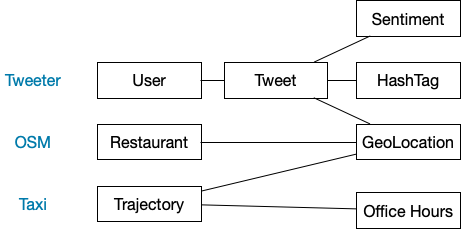
\includegraphics[width=\linewidth,height=\textheight,keepaspectratio]{images/Sample_Data}
  \caption{Original Dataset}
  \label{sample_data}
\end{figure}

\subsection{Graph Translation Algorithm}
\begin{figure}[!htbp]
  \centering
  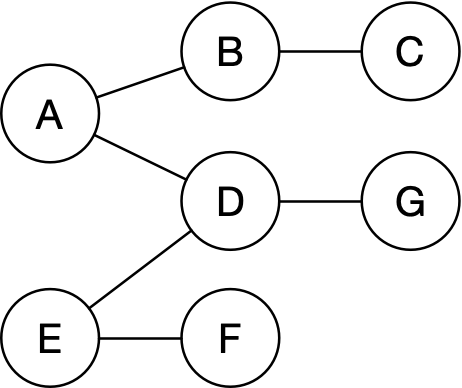
\includegraphics[width=100pt,keepaspectratio]{images/Sample_Graph}
  \caption{Graph Example}
  \label{graph_model}
\end{figure}

\begin{figure}[!htbp]
  \centering
  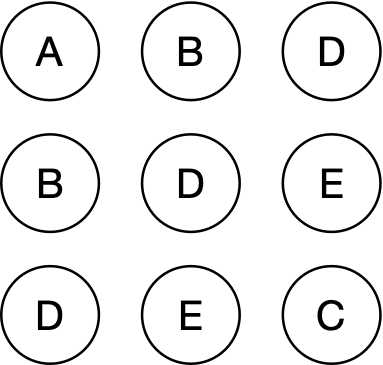
\includegraphics[width=100pt,keepaspectratio]{images/n-gram-grah}
  \caption{N-Gram Model}
  \label{n_gram_graph}
\end{figure}
In order to create neighbourhood matrix that represents vertex in consistent order we used sorting algorithm based on in-degree and out-degree of nodes. First, part is to create sub-graph that is represents context of node entities. In order to generate sub-graph, we first visit each neighboring node and compare depth from starting node to connected edges of visiting node which becomes terminating factor for sub-graph.
\subsection{Graph Convolutional Layer}

\subsection{Capsule Layer}
% \begin{figure}
% \begin{tikzpicture}[scale=1.8, auto,swap]
%     % Draw a 7,11 network
%     % First we draw the vertices
%     \foreach \pos/\name in {{(0,2)/a}, {(2,1)/b}, {(4,1)/c},
%                             {(0,0)/d}, {(3,0)/e}, {(2,-1)/f}, {(4,-1)/g}}
%         \node[vertex] (\name) at \pos {$\name$};
%     % Connect vertices with edges and draw weights
%     \foreach \source/ \dest /\weight in {b/a/7, c/b/8,d/a/5,d/b/9,
%                                          e/b/7, e/c/5,e/d/15,
%                                          f/d/6,f/e/8,
%                                          g/e/9,g/f/11}
%         \path[edge] (\source) -- node[weight] {$\weight$} (\dest);
%     % Start animating the vertex and edge selection. 
%     \foreach \vertex / \fr in {d/1,a/2,f/3,b/4,e/5,c/6,g/7}
%         \path<\fr-> node[selected vertex] at (\vertex) {$\vertex$};
%     % For convenience we use a background layer to highlight edges
%     % This way we don't have to worry about the highlighting covering
%     % weight labels. 
%     \begin{pgfonlayer}{background}
%         \pause
%         \foreach \source / \dest in {d/a,d/f,a/b,b/e,e/c,e/g}
%             \path<+->[selected edge] (\source.center) -- (\dest.center);
%         \foreach \source / \dest / \fr in {d/b/4,d/e/5,e/f/5,b/c/6,f/g/7}
%             \path<\fr->[ignored edge] (\source.center) -- (\dest.center);
%     \end{pgfonlayer}
% \end{tikzpicture}
% \end{figure}

\FloatBarrier
\subsection{Training}

\begin{figure}[!htbp]
  \centering
  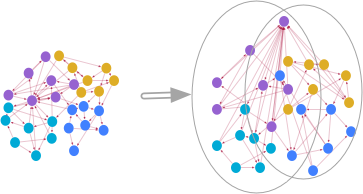
\includegraphics[width=\linewidth,height=\textheight,keepaspectratio]{images/graph_normalization}
  \caption{Graph Representation Model}
  \label{graph_model}
\end{figure}